\documentclass[11pt,a4paper]{article}
\usepackage[utf8]{inputenc}
\usepackage[T1]{fontenc}
\usepackage[english]{babel}
\usepackage[margin=2.1cm]{geometry}
\usepackage{booktabs,array,tabularx}
\usepackage{xcolor}
\usepackage{graphicx}
\usepackage{pgfplots}
\pgfplotsset{compat=1.17}
\PassOptionsToPackage{hyphens}{url}
\usepackage[hidelinks]{hyperref}
\usepackage{enumitem}
\setlist{nosep,leftmargin=1.4em}
\emergencystretch=3em

\definecolor{impl}{HTML}{3B6EA8}
\definecolor{rev}{HTML}{8FB3DA}
\definecolor{waste}{HTML}{C0504D}

\title{Sweatshop on P-Chess: lane \texttt{core}, early morning\\\large Input modes, premoves, history, review screen, openings, Lc0 failures and the flag race (10 tickets); GPT-6.1 Sol lineup}
\author{Foreman, session \texttt{sweatshop/core/2026-10-25-0159}}
\date{25 October 2026}

\begin{document}
\maketitle

\section*{Summary}

Lane \texttt{core} ran in the clone \path{.artifacts-build/lanes/core}, from \texttt{main} at
\texttt{5ee5836} (PRs \#8 and \#9 merged). Bruno authorized the relaunch with the
\texttt{gpt-6.1-sol} lineup (``Pode relançar a lane core com a lineup gpt-6.1-sol''): one
launch at 01:59, \texttt{-Models 'stage 2 gpt-6.1-sol high, hard gpt-6.1-sol xhigh, stage 3
gpt-6.1-sol xhigh'} (logged by the driver as \texttt{ad hoc}; the same models as the
\texttt{Models:} binding), pid 21760, all stages on Codex. No \texttt{STOP} was asked for; the
driver ended at 06:12 with ``Nothing runnable''. The standup expected five ready tickets
(UI-006, UI-007, HIST-001, OPEN-001, BOT-008); each merge unblocked the next, so the run also
took HIST-002, OPEN-002, OPEN-003, OPEN-004, and CLOCK-002 once Bruno chose its test seam
mid-run.

\begin{itemize}
  \item \textbf{Produced:} \textbf{10 tickets approved and merged on the session} PR
        \href{https://github.com/Laginho/P-Chess/pull/10}{\#10}: UI-006, UI-007, HIST-001,
        HIST-002, OPEN-001, OPEN-002, OPEN-003, OPEN-004, BOT-008, CLOCK-002, all
        \texttt{Review: agent}, \texttt{Verdict: Approve}, no \emph{Needs your call}. Gate at
        the last merge: 235 passed, 0 failed (from 152 before the run).
  \item \textbf{Cost:} \textbf{\$25.44} at API list price over 28 stages, all priced:
        \texttt{gpt-6.1-sol xhigh} \$15.52 (\$12.11 in review, \$3.41 as hard implementer),
        \texttt{gpt-6.1-sol high} \$9.92. Codex quota: 26 points of the weekly window
        (\texttt{gpt-6.1-sol xhigh} 13, about 10 in review and 3 as hard implementer;
        \texttt{gpt-6.1-sol high} 11; 2 outside the stages). Section Codex quota has the
        detail.
  \item \textbf{What went wrong:} four tickets came back once each (UI-007, HIST-001,
        OPEN-001, OPEN-003), every one for a real miss against an explicit criterion; the four
        reopen rounds cost \$5.95, 23\% of the run. Nothing crashed, nothing was parked, and the
        foreman made no cleanup.
  \item \textbf{Provisional verdict:} the cheapest run of the project per ticket, \$2.54 per
        approved ticket against \$7.20--\$8.30 for the Opus core runs. Reviews were short
        (median 5~min) and still caught each reopen with a reproduction. Manual product
        acceptance is pending on most tickets, and one known defect (Maia moving at zero,
        CLEAN-005) remains a release condition.
\end{itemize}

\section*{What was done}

\textbf{UI-006}: the board takes moves by clicking a piece and then a square (an option, off
by default), auto-queens promotions (off / on / only on premoves; \texttt{Alt} opens the picker
anyway), and draws arrows with a right-drag and circles with a right click; a left click
clears them. Mostly \path{ui/board_view.gd}; the shared promotion rule is
\texttt{PromotionPicker.should\_auto\_queen}. Drawing while Maia is to move was handed to
UI-007.

\textbf{UI-007}: premoves. While Maia thinks the player can queue moves, shown as ghost pieces;
Lichess style holds one, Chess.com style a queue; each due premove plays at once, costs 0.1~s
and plays its sound; an illegal one drops the rest; a right click cancels. New
\path{ui/premove_queue.gd}. Reopened once: the ghost check let a queued move capture Black's
king (\texttt{e2e4}, then \texttt{f1c4 d1h5 h5f7 f7e8}), because the queue replayed the human's
moves with the ordinary generator, which never expects a king to be capturable. The real game
was safe (the due move is checked again); the queue now refuses king captures.

\textbf{HIST-001}: every finished game is saved as a PGN with the clock after each move, and
results are counted per Maia level and time control. New \path{core/history.gd}. Reopened
once: the settings-screen test started the real game scene without a private history folder,
so the new start-up code read the player's own \path{user://stats.cfg}; the test now gets an
isolated history.

\textbf{HIST-002}: when a game ends, a review screen shows the result and the time spent on
every move, and exports the game as PGN or opens it on Lichess, with rematch and back to setup.
New \path{ui/review.gd}. The first move of each side shows 0~ms (a first premove 100~ms),
following CLOCK-001's untimed first move.

\textbf{OPEN-001}: the full Lichess opening catalog (3,865 lines, CC0, pinned upstream commit)
loads into a searchable tree with checkboxes, and selections can be saved by name for the
Catalog mode. \path{bot/book.gd}, \path{ui/opening_picker.gd}. Reopened once: search ran on
the tree's rebuilt names, in which \path{bot/book.gd} had rewritten the punctuation, so typing
an original name with a comma or colon found nothing (46 lines, e.g. ``Polish Opening, with
d5''). The first catalog load takes about 17~s on a background thread; later openings reuse it.

\textbf{OPEN-002}: Maia now prefers the checked catalog lines early in the game and fades back
to her own play later, with a configurable intensity; positions reached by transposition count;
practice counts persist and saved games get an \texttt{Opening} header. \path{bot/book.gd},
\path{bot/maia\_player.gd}. Five scripted games against the real Lc0 confirmed the early
preference and the fade.

\textbf{OPEN-003}: a player's repertoire can be imported from a PGN (Lichess study chapters,
variations, comments), merged into one move tree and played in ``My repertoire'' mode with the
saved colour (rematches swap colours). New \path{bot/repertoire.gd} and an import dialog.
Reopened once: comments written before a chapter's first move were dropped from the merged
tree.

\textbf{OPEN-004}: the review screen marks book moves, repertoire moves and the move where the
player left the repertoire, with the expected continuation in SAN; the check can be switched
off in every mode. New \path{bot/badges.gd}.

\textbf{BOT-008}: if Lc0 dies or rejects the Maia net, the game stops and returns to the setup
screen with the error, instead of waiting forever. \path{engine/uci.gd}; an \texttt{error}
line from Lc0 now counts as fatal even after \texttt{readyok}, because Lc0 v0.32.1 rejects a
missing net and keeps running.

\textbf{CLOCK-002}: a piece dropped in the same frame the player's clock reached zero no longer
plays; the clock is ticked before the board handles input (\path{ui/main.gd}, seven lines),
using the test seam Bruno chose (the real game scene under the test runner, with a fake time
source).

\section*{Timeline}

\begin{tabularx}{\linewidth}{@{}lX@{}}
\toprule
01:59 & Clone fast-forwarded to \texttt{5ee5836}; standup: five ready, CLOCK-002 blocked, tree clean, no driver. Launch, pid 21760, session \texttt{sweatshop/core/2026-10-25-0159}. \\
02:18 & UI-006 merged, 0 findings. Bruno (relayed) unblocks CLOCK-002 with seam (a); the foreman commits the contract on the session by plumbing during UI-007's stage 2 (\texttt{b206a36}). \\
02:45 & UI-007 reopened (king capture in the ghost). 02:58 merged. \\
03:13 & HIST-001 reopened (settings test reads the player's stats). 03:22 merged. \\
03:38 & HIST-002 merged, 0 findings. \\
04:04 & OPEN-001 reopened (search loses punctuation). 04:15 merged. \\
04:42 & OPEN-002 (hard) merged, 0 findings. \\
05:04 & OPEN-003 reopened (chapter comments dropped). 05:11 merged. \\
05:33 & OPEN-004 merged, 0 findings. 05:54 BOT-008 merged, 0 findings. \\
06:12 & CLOCK-002 merged, 0 findings; ``Nothing runnable''; PR \#10 updated (10 tickets). \\
\bottomrule
\end{tabularx}

\section*{Per stage}

{\small
\begin{tabularx}{\linewidth}{@{}llllrrrrrX@{}}
\toprule
When & Ticket & Stage & Model & Min & In & Cache & Out & Cost & Outcome \\
\midrule
02:13 & UI-006 & impl & sol high & 12 & 2.8M & 95\% & 21k & 1.03 & to-review \\
02:18 & UI-006 & review & sol xhigh & 5 & 2.1M & 90\% & 13k & 0.92 & merged \\
02:40 & UI-007 & impl & sol xhigh & 22 & 4.0M & 98\% & 34k & 1.30 & to-review \\
02:45 & UI-007 & review & sol xhigh & 6 & 3.0M & 91\% & 16k & 1.26 & reopened \\
02:52 & UI-007 & impl & sol xhigh & 6 & 1.6M & 95\% & 10k & 0.56 & to-review \\
02:58 & UI-007 & review & sol xhigh & 6 & 1.9M & 93\% & 13k & 0.73 & merged \\
03:09 & HIST-001 & impl & sol high & 11 & 2.9M & 95\% & 22k & 1.06 & to-review \\
03:13 & HIST-001 & review & sol xhigh & 4 & 1.8M & 90\% & 10k & 0.79 & reopened \\
03:18 & HIST-001 & impl & sol high & 4 & 1.2M & 91\% & 8k & 0.50 & to-review \\
03:22 & HIST-001 & review & sol xhigh & 5 & 1.5M & 91\% & 11k & 0.65 & merged \\
03:34 & HIST-002 & impl & sol high & 11 & 2.4M & 93\% & 21k & 0.96 & to-review \\
03:38 & HIST-002 & review & sol xhigh & 5 & 2.1M & 92\% & 13k & 0.85 & merged \\
03:57 & OPEN-001 & impl & sol high & 18 & 3.6M & 98\% & 30k & 1.19 & to-review \\
04:04 & OPEN-001 & review & sol xhigh & 8 & 3.0M & 94\% & 16k & 1.08 & reopened \\
04:10 & OPEN-001 & impl & sol high & 6 & 1.3M & 94\% & 7k & 0.47 & to-review \\
04:15 & OPEN-001 & review & sol xhigh & 5 & 1.7M & 93\% & 10k & 0.65 & merged \\
04:36 & OPEN-002 & impl & sol xhigh & 21 & 4.0M & 95\% & 37k & 1.55 & to-review \\
04:42 & OPEN-002 & review & sol xhigh & 6 & 3.1M & 93\% & 15k & 1.14 & merged \\
04:58 & OPEN-003 & impl & sol high & 16 & 3.7M & 97\% & 32k & 1.29 & to-review \\
05:04 & OPEN-003 & review & sol xhigh & 5 & 2.5M & 92\% & 13k & 0.99 & reopened \\
05:07 & OPEN-003 & impl & sol high & 3 & 0.8M & 94\% & 5k & 0.30 & to-review \\
05:11 & OPEN-003 & review & sol xhigh & 4 & 1.4M & 90\% & 10k & 0.62 & merged \\
05:27 & OPEN-004 & impl & sol high & 16 & 3.0M & 95\% & 29k & 1.15 & to-review \\
05:33 & OPEN-004 & review & sol xhigh & 6 & 2.1M & 92\% & 12k & 0.84 & merged \\
05:50 & BOT-008 & impl & sol high & 17 & 3.7M & 96\% & 22k & 1.21 & to-review \\
05:54 & BOT-008 & review & sol xhigh & 4 & 2.2M & 91\% & 11k & 0.88 & merged \\
06:04 & CLOCK-002 & impl & sol high & 10 & 2.3M & 96\% & 14k & 0.77 & to-review \\
06:12 & CLOCK-002 & review & sol xhigh & 7 & 1.8M & 93\% & 12k & 0.72 & merged \\
\midrule
 & & & & 249 & 67.5M & & 467k & 25.44 & \\
\bottomrule
\end{tabularx}
}

\smallskip
{\small ``sol'' is \texttt{gpt-6.1-sol}. UI-007 and OPEN-002 ran on the hard implementer
(\texttt{Difficulty: hard}).}

\begin{center}
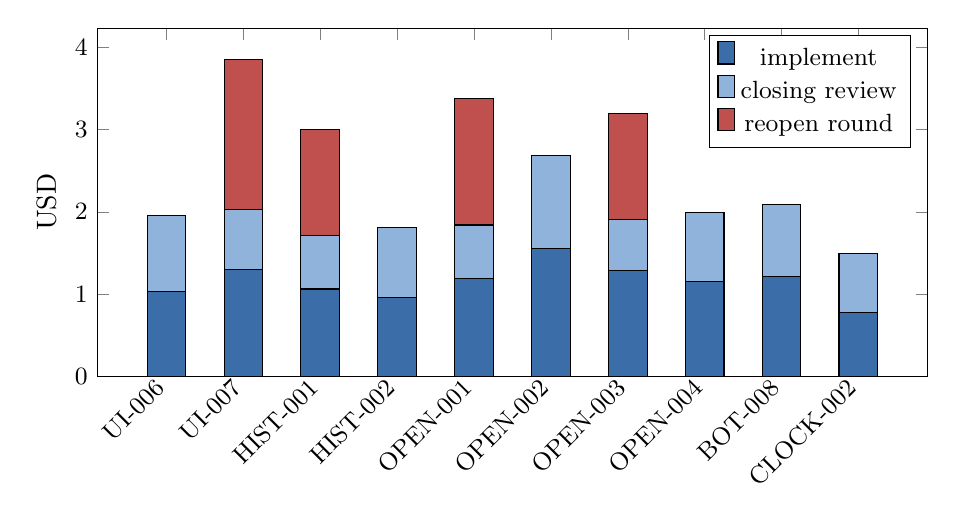
\begin{tikzpicture}
\begin{axis}[ybar stacked, bar width=14pt, width=\linewidth, height=6cm,
  symbolic x coords={UI-006,UI-007,HIST-001,HIST-002,OPEN-001,OPEN-002,OPEN-003,OPEN-004,BOT-008,CLOCK-002},
  xtick=data, x tick label style={rotate=45,anchor=east,font=\small}, ylabel={USD}, ymin=0,
  legend style={at={(0.98,0.98)},anchor=north east,font=\small}, tick label style={font=\small}]
\addplot[fill=impl] coordinates {(UI-006,1.03) (UI-007,1.30) (HIST-001,1.06) (HIST-002,0.96) (OPEN-001,1.19) (OPEN-002,1.55) (OPEN-003,1.29) (OPEN-004,1.15) (BOT-008,1.21) (CLOCK-002,0.77)};
\addplot[fill=rev] coordinates {(UI-006,0.92) (UI-007,0.73) (HIST-001,0.65) (HIST-002,0.85) (OPEN-001,0.65) (OPEN-002,1.14) (OPEN-003,0.62) (OPEN-004,0.84) (BOT-008,0.88) (CLOCK-002,0.72)};
\addplot[fill=waste] coordinates {(UI-006,0) (UI-007,1.82) (HIST-001,1.29) (HIST-002,0) (OPEN-001,1.54) (OPEN-002,0) (OPEN-003,1.29) (OPEN-004,0) (BOT-008,0) (CLOCK-002,0)};
\legend{implement, closing review, reopen round}
\end{axis}
\end{tikzpicture}
\end{center}

The red segments are the four reopen rounds (the review that sent the ticket back plus the
retry), \$5.95 in all. Every retry was small (3--6~min, \$0.30--\$0.56): the findings were
narrow and came with a reproduction. Input is 90--98\% cache reads; the costliest stage was
OPEN-002's hard implementation (\$1.55).

\section*{Comparison with previous runs}

From \texttt{run-log.md}: lane \texttt{core} on Opus cost \$7.20 per approved ticket (night) and
\$8.30 (afternoon); the UI-004/UI-005 runs and their reworks \$23.01 for two tickets; lane
\texttt{mvp} on this same lineup \$2.69. This run: \$2.54 (\$25.44 over 10). Stage 2 took
3--22~min (median 11.5) and reviews 4--8~min (median 5), against 12--29~min for Opus high on
the afternoon run. The reopen rate was 4 of 14 reviews (29\%), above the lineup's history
(16\% before this run); every reopen was a single narrow finding.

\section*{Codex quota}

From \texttt{codex-quota.ps1} over the run's window (01:59--06:13), baseline 25\% at 01:54.
The total is exact; one stage is $\pm$1 point, since Codex rounds to integers. The script
flags a weekly-window boundary during UI-007's first review, so that stage's point may be
misread.

\begin{center}
\begin{tabular}{@{}lrr@{}}
\toprule
Model and role & Cost (USD) & Weekly quota \\
\midrule
\texttt{gpt-6.1-sol high}, stage 2 & 9.92 & 11 points \\
\texttt{gpt-6.1-sol xhigh}, stage 3 & 12.11 & about 10 points \\
\texttt{gpt-6.1-sol xhigh}, hard stage 2 (UI-007, OPEN-002) & 3.41 & about 3 points \\
Outside the stages (8 threads) & -- & 2 points \\
\midrule
Run total & 25.44 & 26 points \\
\bottomrule
\end{tabular}
\end{center}

The 8 threads outside the stages are other Codex work in the same account during the window
(the stages' \texttt{gpt-6-astra} proxy calls run inside their stage).

\section*{Observations per model}

\begin{itemize}
  \item \textbf{gpt-6.1-sol high, stage 2 (8 tickets, 11 runs)}: test first in every cycle,
        with separate test and production commits and red results recorded; every handoff
        named what it did not check (visual, audio, clipboard, browser). It asked the proxy
        whenever a fix needed a file outside Primary files, instead of editing it. Its three
        reopens were each a path it did not walk: one more caller of the new start-up code
        (HIST-001), searching the names it had itself rewritten (OPEN-001), and a comment
        position in its own parser's output (OPEN-003).
  \item \textbf{gpt-6.1-sol xhigh, hard stage 2 (UI-007, OPEN-002)}: the two largest
        tickets, 21--22~min each. UI-007 reconciled UI-006's handoff (drawing during Maia's
        turn) without being reminded; it missed the king-capture case in the ghost board.
        OPEN-002 passed review at once, with five real-engine games as acceptance.
  \item \textbf{gpt-6.1-sol xhigh, review (14 reviews)}: 10 merges, 4 reopens, each with a
        reproduction and the exact lines; no code authored in review, so no round-0 rows. It
        filed five follow-up tickets for things outside the criteria (CLEAN-002 to CLEAN-006)
        instead of leaving notes in closed tickets, which keeps them visible.
\end{itemize}

\section*{Driver and runtime issues}

\begin{enumerate}
  \item \textbf{None blocking.} No crash, no park, no failed attempt; every stage ran on
        Codex and produced its gate receipt with \path{gate-evidence.ps1}.
  \item \textbf{A ticket unblocked mid-run.} Bruno chose CLOCK-002's seam while the driver
        ran. The driver reads tickets from the session ref at every loop, so the foreman
        committed the contract with Git plumbing (\texttt{commit-tree} and a compare-and-swap
        \texttt{update-ref}) while the clone sat on UI-007's ticket branch, and pushed it. The
        driver picked CLOCK-002 up after BOT-008 without a relaunch.
  \item \textbf{Scene tests multiply.} Five tickets added start-up work to the real game
        scene, and three of them had to adapt other tickets' scene-test helpers (HIST-001,
        OPEN-002, OPEN-003), each by a proxy decision. The gate grew from 152 to 235 tests.
\end{enumerate}

\section*{Recommendations}

\begin{enumerate}
  \item Keep the gpt-6.1-sol lineup for lane \texttt{core}: \$2.54 per ticket. Scoreboard
        rows: \texttt{gpt-6.1-sol high} $\rightarrow$ \texttt{gpt-6.1-sol xhigh} 102 reviews,
        16\% reopened, S2 rate 15\%; \texttt{opus-5.5 high} $\rightarrow$
        \texttt{opus-5.5 xhigh} 12 reviews, 17\% (a small sample, at about three times the cost
        per ticket).
  \item Stage 1 should triage the five CLEAN tickets the reviews filed. CLEAN-005 (Maia's move
        can land at zero) is a release condition; CLEAN-006 holds the real-Main rematch tests
        UI-004 still owes.
  \item When a ticket adds start-up code to the main scene, its stage 2 should grep every test
        that instantiates \path{ui/main.tscn}. HIST-001's reopen came from the one caller it
        missed, and OPEN-002 then had to touch four scene-test helpers.
  \item The 17~s first catalog load is not under any criterion. If it bothers Bruno in play,
        a cached parse of the five TSVs is a small follow-up.
\end{enumerate}

\section*{Human debt and proxy decisions}

No \texttt{Débito humano:} lines this run. Bruno decided twice, relayed by the supervising
session: relaunch lane \texttt{core} on the gpt-6.1-sol lineup; and CLOCK-002's test seam,
option (a) (``pode destravar o clock-002 também, aceito sua sugestão''). Every
\texttt{Proxy decided} line of the run is \texttt{(gpt-6-astra high, fallback)}, 12 in all:

\begin{itemize}
  \item \textbf{UI-006}: add the two Main settings routes and criterion-focused tests; retain
        the existing turn-input lock for UI-006, leaving opponent-turn input integration with
        UI-007.
  \item \textbf{UI-007} (written during review): reopen for criterion 2; queued moves must not
        capture the opposing king in the ghost position; unknown Maia replies are handled by
        execution-time revalidation and do not excuse accepting an invalid move.
  \item \textbf{HIST-001}: isolated History harnesses in \path{test_session.gd} and
        \path{test_premove.gd} plus the real-Main history integration seam.
  \item \textbf{HIST-001}: isolated History injection, storage lifecycle and a start-up
        identity assertion in \path{test_input_modes.gd}, preserving its settings assertions.
  \item \textbf{HIST-002}: criterion 2 reconstructs charged time using only awarded
        increments, preserving 100~ms first premoves and zero-clock snapshots without
        increment; scene tests in \path{tests/test_review.gd}.
  \item \textbf{OPEN-002}: narrowly scoped Main lifecycle wiring and scene tests in
        \path{test_book.gd}; criterion 7 clarified to allow positional re-entry.
  \item \textbf{OPEN-002}: \path{opening_picker.gd} gets one shared public asynchronous
        catalog-readiness entry point used by Main and \texttt{present()}.
  \item \textbf{OPEN-002}: tiny preloaded-catalog injection in the \texttt{\_session} helpers
        of four existing scene-test files, assertions unchanged.
  \item \textbf{OPEN-003}: Main repertoire lifecycle wiring and real-scene tests; the imported
        colour for setup starts, the actual game colour for rematches.
  \item \textbf{OPEN-003}: update only OPEN-001's temporary ``My repertoire disabled''
        assertion to expect the mode enabled.
  \item \textbf{OPEN-004}: Main composition wiring; the Book badge independent of the
        repertoire toggle; only the first unmatched human move marked, with explicit
        no-continuation text.
  \item \textbf{BOT-008}: fail closed on Lc0's \texttt{error} output even after
        \texttt{readyok}; exercise missing weights through the next policy request.
\end{itemize}

\section*{Feature acceptance}

Against the milestones in \path{docs/spec.md}, reusing the stages' evidence on identical code:

\begin{itemize}
  \item \textbf{M5} (every setting works and persists; UI-005, UI-006, UI-007): automated
        persistence and input tests pass; \emph{pending} the manual checks (gesture feel,
        ghosts, premove audio).
  \item \textbf{M6} (badges and times correct on saved games; HIST-001, HIST-002, with
        OPEN-004's badges): automated real-Main games and saved-PGN checks pass;
        \emph{pending} two interactive games, the real clipboard and the Lichess import.
  \item \textbf{M7} (Maia follows the chosen lines and drifts off them; OPEN-001 to OPEN-004):
        \emph{passed} on automated evidence, five scripted games against the real Lc0
        (OPEN-002) and real Maia-1500 repertoire play (OPEN-003); the visual check is pending.
  \item \textbf{M4} addition (CLOCK-002): \emph{passed} headless through real viewport input.
        Known deferred defect: Maia's own move can still land at zero (CLEAN-005), a release
        condition.
\end{itemize}

\section*{Reopen attribution}

Four reopened reviews, one finding each; judged by the foreman (Opus), since the reviewer is
\texttt{gpt-6.1-sol}. No merging review authored a fix, so no round-0 rows. PR \#10 has no
review findings yet; no session-review, release-audit or post-release discovery this run.

{\small
\noindent\begin{tabularx}{\linewidth}{@{}lcXp{2.3cm}X@{}}
\toprule
Ticket & Rnd & Finding & Label & Why \\
\midrule
UI-007 & 1 & Ghost validation accepted capturing the opposing king & S2-explícito/\allowbreak código & Criterion 2: each premove checked against the position after the queued ones. \\
HIST-001 & 1 & Settings test's real Main read the player's \path{stats.cfg} & S2-explícito/\allowbreak código & Criterion 7: every automated Main test uses isolated history; a regression of stage 2's own start-up code. \\
OPEN-001 & 1 & Search lost original punctuation (46 lines) & S2-explícito/\allowbreak código ? & Criterion 4: substring search; borderline as the criterion does not say original or displayed names. \\
OPEN-003 & 1 & Chapter-leading comments not merged into the tree & S2-explícito/\allowbreak código & Criterion 1: every chapter's comments merge into one tree. \\
\bottomrule
\end{tabularx}
}

\smallskip
Totals: S2-explícito/código 4 (one borderline). Review miss: none (all first reviews). Churn:
none.

\section*{Scoreboard}

\texttt{scoreboard.ps1} over P-Chess, ClassyCall, EasyMath, PhysiSyst, SIGAA-ME, SynchroNice and
slip. For P-Chess the lane clone was read instead of the main checkout, after the merged log was
copied back to both: the clone also holds this run's uncommitted attribution and intervention
rows, and one P-Chess path is read, so no row counts twice. Rows that moved since the previous
\texttt{core} report: \texttt{gpt-6.1-sol high} $\rightarrow$ \texttt{gpt-6.1-sol xhigh} 89
$\rightarrow$ 102 reviews, 12 $\rightarrow$ 16 reopened (13\% $\rightarrow$ 16\%), S2 11
$\rightarrow$ 15; a new row \texttt{gpt-6.1-sol xhigh} $\rightarrow$ \texttt{gpt-6.1-sol xhigh},
4 reviews, 1 reopened (an anecdote); \texttt{opus-5.5 high} $\rightarrow$ \texttt{opus-5.5
xhigh} 8 $\rightarrow$ 12 (the UI-004/UI-005 runs).

{\small
\begin{tabular}{@{}llrrrrrr@{}}
\toprule
Implementer & Reviewer & Reviews & Reopened & Rate & S2 & S2 rate & Fixed in rev. \\
\midrule
gpt-6.1-sol high & gpt-6.1-sol xhigh & 102 & 16 & 16\% & 15 & 15\% & 6 \\
gpt-6.1-sol high & gpt-6.1-sol max & 94 & 21 & 22\% & 20 & 21\% & 4 \\
gpt-6.1-sol xhigh & gpt-6.1-sol xhigh & 4 & 1 & 25\% & 1 & 25\% & 1 \\
opus-5.5 high & opus-5.5 xhigh & 12 & 2 & 17\% & 2 & 17\% & 4 \\
opus-5.5 xhigh & opus-5.5 xhigh & 8 & 0 & 0\% & 0 & 0\% & 0 \\
? & opus-5.5 xhigh & 4 & 1 & 25\% & 1 & 25\% & 0 \\
\bottomrule
\end{tabular}
}

\medskip
Implementers: \texttt{gpt-6.1-sol high} 229 runs, 200 to review, 8 failed, 21 asked, median
19~min, \$380.59; \texttt{gpt-6.1-sol xhigh} 4 runs, all to review, \$4.74. Discoveries:
252 ticket-review findings, 13 session-review (9 of 10 known were earlier review misses).
Interventions across repos: 24 human rescues, 61 automatic recoveries, 14 routine approvals,
44 \texttt{gpt-6-astra high, fallback}, 29 Opus and 12 supervisor proxy decisions, 37 unknown.
Runtime completion to process exit: 917~s over 669 measured stages, 763 unmeasured.

\section*{Pending for the human}

\begin{enumerate}
  \item Review and merge PR \#10 (10 tickets); then tell the other open lanes' foremen to
        sync.
  \item Manual checks: UI-006 (click-click, promotion, arrows), UI-007 (a 1+0 game with
        premoves, ghosts, audio), HIST-001 (two games, then open their PGNs in
        \path{user://games/}), HIST-002 (copy the PGN, open on Lichess, compare), BOT-008
        (kill Lc0 in Task Manager mid-game), plus the visual look of the opening picker,
        repertoire import and review badges.
  \item Stage 1: triage CLEAN-002 to CLEAN-006; CLEAN-005 (Maia's move at zero) is a release
        condition.
  \item Carried over: UI-004 and UI-005 manual checks, BOT-004's latency on an idle machine,
        CLOCK-001's manual games, \texttt{PolicyTemperature}.
\end{enumerate}

\end{document}
